\cotefile{156-7}
\scanpage{101}
\handwritten{
\mspage{100}
% Two vertical emphasis strokes beside the corollary.
\margin{$\Vert$\quad ?}
\uline{Corollaire} $\forall Z\in\unsure{\mathcal M|M}$ tel que \inserted{$\forall X'\in\widetilde F^{\circ}$, on ait} $Z\parallel\deleted{X}\operatorname{omb}(X')^{\circ}$ et \deleted{\unsure{Alors soit}} $Z\parallel\unsure{\operatorname{omb}|\operatorname{int}}(X)^{\circ}$.

\inserted{\uline{Par \unsure{At L2}}} On est ramené au cas où $Z=x\in\unsure{\mathcal L|L}$.

Je rappelle que $F\preccurlyeq X$ signifie $F\ll X$ et $\operatorname{supp}. F=\mathrm{s}\text{-}\unsure{\mathscr W|W}X$. Si on a une fonction $\deleted{\unsure{\mathrm{s}\text{-}\mathscr W X}}\inserted{X\longrightarrow |X|}$ à valeurs dans un \unsure{ens.} $P$ (cf. p.\,80, condition $\mathrm{S}\text{-}\mathscr W_{\unsure{\phi|p}}1$ -- \unsure{ou|on} un $\mathrm{s}\text{-}\mathscr W$-\unsure{inv} par $\mathrm{S}\text{-}\mathscr W_{\phi}2$) alors pour $F\ll X$, la condition $F\preccurlyeq X$ signifie simplement que $\deleted{\unsure{\partial}}|F|=|X|$. Je dis que \deleted{\unsure{les}}
% margin note written sideways / slanted
\margin{On doit $\mathrm{s}\text{-}\mathscr W$ \unsure{non} \unsure{coW} $\unsure{K\longleftrightarrow X|K\ll X}$.}
\[
\left\{\begin{aligned}
\text{\textcircled{a}}\quad \deleted{\unsure{\operatorname{supp}}}\quad |X^{\circ}|&=|X|\setminus|\partial X|,\quad\text{et que}\\
\text{\textcircled{b}}\quad \deleted{\unsure{\widetilde F\preccurlyeq F}}\quad \widetilde F^{\circ}&=\{X'\in\widetilde F\mid |X'^{\circ}|\subset|X^{\circ}|\}\\
&=\{X'\in\widetilde F\mid |X'^{\circ}|\cap|X^{\circ}|\ne\varnothing\}
\end{aligned}\right.
\]
\margin{$\unsure{B}$}

Comme $X^{\circ}\parallel\partial X$, \deleted{\unsure{on a}} et $X^{\circ}\subset\deleted{X}\inserted{\mathrm{s}\text{-}\mathscr W X}$, on a $|X^{\circ}|\subset|X|=|\mathrm{s}\text{-}\mathscr W X|$, et $|X^{\circ}|\cap|\partial X|=\varnothing$, donc
\[
\unsure{=|\Rightarrow}\quad |X^{\circ}|\subset|X|\setminus|\partial X|
\]
% Two horizontal separator strokes above the reused typescript.
\figure{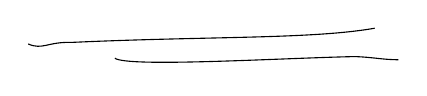
\begin{tikzpicture}[x=1cm,y=1cm]
\draw (0,0.20) .. controls (0.18,0.12) and (0.25,0.23) .. (0.55,0.22) .. controls (2.3,0.30) and (3.6,0.26) .. (4.4,0.40);
\draw (1.10,0.02) .. controls (1.25,-0.10) and (3.2,0.02) .. (4.15,0.04) .. controls (4.4,0.03) and (4.5,0.00) .. (4.7,0.00);
\end{tikzpicture}}
}
% Reused typescript below is upside down relative to the manuscript.
% Three diagonal cancellation strokes pass through the whole typed block.
\mspage{\deleted{A 6}}
\deleted{de "mot de la fin", pas de "conclusions" dans Récoltes et Semailles; pas plus qu'il n'y en a dans ma vie, ou dans la tienne. Il y a un vin, vieilli pendant une vie dans les fûts de mon être. Le dernier verre que tu boiras ne sera pas meilleur que le premier ou que le centième . Ils sont tous "le même", et ils sont tous différents. Et si le premier verre est gâté, tout le tonneau l'est ; autant alors boire de la bonne eau (s'il s'en trouve), plutôt que du mauvais vin.}

\deleted{Mais un bon vin ne se boit pas à la va-vite, ni au pied levé.}
\scanpage{102}
\mspage{101}
J'ai envie de prendre sur un ``\unsure{magasin}'' $(\unsure{\mathcal M|M},\leq,\ll\ldots)$ comme relation primitive, en plus de $\leq$ et de $\ll$, et au lieu de $\unsure{\gtrless|\bowtie}$ ou de $\parallel$, la \deleted{\unsure{la}} relation
% The parenthesis is added immediately above the equivalence sign.
\inserted{(heuristiquement)}
\[
X\mathrel{|\circ|}Y\quad\Longleftrightarrow\quad X^{\circ}\parallel Y^{\circ}
\]
et ceci de façon à arriver à donner un sens raisonnable à $X^{\circ}$, même dans des cas où au sens plus \unsure{précis} \unsure{présent} elle serait vide. \deleted{\unsure{C}} Cf p.\,53 pour un exemple : \deleted{\unsure{pour}} une maquette simpliciale, plus gén. un ensemble ordonné $(\mathcal M,\leq)$ (où on prend $\ll=\leq$, $X\gtrless Y$ tjs satisfait) \deleted{\unsure{du} \inserted{\unsure{type}} \unsure{quel|que le} \unsure{dont} \unsure{l'élément} \unsure{minimum} \unsure{est le} \unsure{sommet} \unsure{de} $\unsure{X}$ \unsure{de} $X\setminus\{X\}$,} Si $X$ \unsure{non} minimum on a $\operatorname{omb}(X)^{\unsure{\partial|\circ|d}}=\varnothing$.

% margin note written sideways / slanted
\margin{$\mathcal M$ partie fermée de $\unsure{\mathscr P|\mathcal P}_{f}(\unsure{S|\mathcal S})$ pour $\subset$, contenant les $\{s\}$.}
Pour une maquette simpliciale $(S,\mathcal M\subset\mathscr P_f(S))$ les supports du $(\mathcal M,\leq,\ll=\leq,\gtrless=\text{tjs satisfait})$, pour la relation $X\parallel Y\ \Longleftrightarrow\ \widetilde X\cap\widetilde Y=\varnothing$ i.e. $X$ et $Y$ non voisins, s'identifient aux parties quelconques de $S$
\[
\Sigma_{\mathcal M}\simeq\mathscr P(S)
\]
le support du \deleted{$\unsure{X\in}$} ``simplexe'' $X$ est $X$ lui $\unsure{=|\equiv}$. Avec la définition plausible
\[
X^{\circ}=\mathrm{s}\text{-}\unsure{\mathscr W|W}X\cap\mathrm{cos}\text{-}\mathscr W\partial X
\]
on trouve $X^{\circ}=\varnothing$ sauf si $X$ \deleted{est} $\in\unsure{\mathcal L|L}$.

C'est triste mais c'est vrai.
\scanpage{103}
\mspage{102}
Je vais prendre comme relations primitives dans $\unsure{\mathcal M|M}$
\[
\leq,\quad\ll,\quad\mathrel{|\circ|}
\]
Avec ça, on va définir $\unsure{\gtrless|\bowtie}$ ainsi (version \deleted{``\unsure{optimiste}''} ``magasin spacieux'', on reviendra bientôt sur la version ``magasin polyédral'') : pour $X,Y\in\mathcal M$, posant $L=\widetilde X\cap\widetilde Y$ \inserted{plus grande partie fermée commune}
\[
X\gtrless Y\quad\Longleftrightarrow\quad\forall X'\in\widetilde X\setminus L,\quad Y'\in\widetilde Y\setminus L,\quad X'\mathrel{|\circ|}Y'
\]
% slanted
\margin{cette définition ne fait pas intervenir $\ll$.}
Nous allons d'abord poser les axiomes Mag $\Lambda1\ldots\inserted{\Lambda\unsure{6|5}}$ (anciennement Prat $\Lambda1\unsure{\text{?}|\S}\ldots$) de la page 51, avec $\Lambda=\mathcal M$.

Mag $\mathcal M1$, Mag $\mathcal M3$, Mag $\mathcal M4$ \unsure{ne varient} \inserted{donnant Mag $1''$, $2''$, $3''$}

Mag $\mathcal M2$ tombe (car \inserted{$\unsure{\mathcal M\Lambda2|\mathrm{M}\Lambda2}$} tautologique si $\Lambda=\mathcal M$)

Mag $\mathcal M5$ \deleted{est tautologique} va résulter du nouvel axiome (remplaçant At L3)
\[
\text{\uline{Mag} }4''\qquad\forall X\in\mathcal M,\ \text{et }Y,Z\leq X,\ \inserted{Y\ne Z,}\ \text{on a}\quad Y\deleted{\unsure{\gtrless}}\mathrel{|\circ|}Z
\]

\diagram{\begin{tikzcd}[ampersand replacement=\&,column sep=small,row sep=small]
\&\&\widetilde X\arrow[dl,dash]\arrow[dr,dash]\&\&\widetilde Y\arrow[dl,dash]\arrow[dr,dash]\&\&\\
\&\widetilde X'\arrow[dr,dash]\arrow[dl,phantom,"\ni" description,sloped]\&\&L\arrow[dl,dash]\arrow[dr,dash]\&\&\widetilde Y'\arrow[dl,dash]\arrow[dr,phantom,"\ni" description,sloped]\&\\
X''\&\&X'_L\arrow[dr,dash]\&\&Y'_L\arrow[dl,dash]\&\&Y''\\
\&\&\&L'\&\&\&
\end{tikzcd}}
Supposons $X\gtrless Y$, soient $X'\unsure{\nleq|\leq}X$, $Y'\leq Y$, prouvons $X'\gtrless Y'$. Introduisons $\longrightarrow$
\[
\begin{aligned}
\deleted{\unsure{X}}L&=\widetilde X\cap\widetilde Y,\quad L'=\widetilde X'\cap\widetilde Y',\quad X'_L=\widetilde X'\cap L=\widetilde X'\cap\widetilde Y,\\
Y'_L&=\widetilde Y'\cap L=\widetilde Y'\cap\widetilde X,\quad\text{donc }L'=X'_L\cap Y'_L.
\end{aligned}
\]
Soit $X''\in\widetilde X'\setminus L'$, $Y''=\widetilde Y'\setminus L'$, prouvons $X''\mathrel{|\circ|}Y''$. Si $X'',Y''\notin L$, cela résulte de l'hypothèse que $\deleted{\unsure{Z}}X\gtrless Y$. Si $X''\in L$ i.e. $X''\in\deleted{\unsure{\widetilde X_L}}\unsure{\widetilde Y}$, ($Y''$ non \unsure{entrant|partant}) alors $X'',Y''\in\widetilde Y$ et $X''\ne Y''$, donc par Mag $4''$ on gagne encore.

Il faut encore \unsure{imposer} Mag $\mathcal M6$ (ex Prat $\Lambda\unsure{6|5}$, pour $\Lambda=\mathcal M$).

Cor. de \uline{Mag} $4''$ Si $X,Y$ avec $X\gtrless Y$, $X\ne Y$, alors $X\mathrel{|\circ|}Y$.
\scanpage{104}
\mspage{103}
On voudra aussi ce qui suit, similaire à ex-Mag $\Lambda5$ :

\uline{Mag} $5''$ La relation $X\mathrel{|\circ|}Y$ est symétrique et \unsure{antiréflexive} i.e. elle implique $Y\mathrel{|\circ|}X$ et $X\ne Y$. De plus, si $X\mathrel{|\circ|}Y$ et $X'\overset{\circ}{\ll}X$, $Y'\overset{\circ}{\ll}Y$ implique $X\mathrel{|\circ|}Y$.

Ceci va impliquer déjà Mag $6$, i.e. si $X,Y\inserted{,Z}\in\unsure{\mathcal M|M}$, $X\unsure{\gtrless|\bowtie}Y$, $Z\ll X,Y$, alors $\exists Z'\in\mathcal M$ avec
\[
Z\ll Z'\leq X,Y.
\]
En effet, par Mag $\mathcal M3$, \deleted{$\unsure{\mathrm{OPS}}\quad Z\overset{\circ}{\ll}X,\ Z\overset{\circ}{\ll}Y$} $\exists X'\in\widetilde X$, $Y'\in\widetilde Y$ avec $Z\overset{\circ}{\ll}X'$, $Z\overset{\circ}{\ll}Y'$. Par \deleted{\unsure{M}} \inserted{Mag $\mathcal M5$} qu'on vient de vérifier, on aura $X'\gtrless Y'$, et par le corollaire de Mag $4''$, on conclut $X'=Y'$, c'est le $Z'$ désiré !

Donc on sait qu'\deleted{\unsure{on}}avec $(\leq,\ll,\gtrless)$ on a un \unsure{atlas}, \deleted{\unsure{Remarque}} donc aussi une relation $\parallel$

\uline{Proposition} 1 Soient $X,Y\in\mathcal M$. Alors
\[
X\parallel Y\quad\Longleftrightarrow\quad\forall X'\in\widetilde X,\ Y'\in\unsure{\overline Y|\widetilde Y},\ \text{on a}\quad X'\mathrel{|\circ|}Y'
\]
En effet, $X\parallel Y$ signifie que \inserted{$X\gtrless Y$ et} $L=\widetilde X\cap\widetilde Y=\varnothing$. \deleted{et $X\gtrless Y$} Donc la prop. est tautologique.

Vérifions At C (\unsure{spac|spec}), i.e.

\uline{Proposition} 2 \inserted{(?)} Soient $X,Y\in\mathcal M$, $L=\widetilde X\cap\unsure{\overline Y|\widetilde Y}$. \deleted{\unsure{Si}} Alors
\[
\begin{aligned}
X\gtrless Y\quad\Longleftrightarrow\quad&\inserted{\text{(condition C)}}\forall X'\ll X,\quad Y'\ll Y,\quad\text{tels que }\deleted{\unsure{X'_L\overset{\mathrm{dfn}}{=}\widetilde X'\cap}}\\
&X'_L\overset{\mathrm{dfn}}{=}\widetilde X'\cap\operatorname{Omb}(L)\quad\text{et }Y'_L\overset{\mathrm{dfn}}{=}\widetilde Y'\cap\operatorname{Omb}(L)\quad\text{soient vides}\\
&\text{on a}\quad X'_{\deleted{\unsure{L}}}\parallel Y'_{\deleted{\unsure{L}}}.
\end{aligned}
\]
$\Longrightarrow$ sûrement toujours vrai, et $\Longleftarrow$ moyennant un axiome \deleted{\unsure{C}} supplémentaire genre At L1 (axiome de divisibilité infinie). Voyons !
\scanpage{105}
\mspage{\unsure{204|104}}
Supposons $X\unsure{\gtrless|\bowtie}Y$, et soient $X'\ll X$, $Y'\ll Y$ avec
\[
X'_L=Y'_L=\varnothing.
\]
prouvons que $X'\parallel Y'$, i.e. \inserted{(prop.\,1)} que \deleted{pour} $\forall X''\leq X'$, $Y''\leq Y'$, on a $X''\mathrel{|\circ|}Y''$. Comme $\deleted{X''}X''_L\leq X'_L=\varnothing$ et \deleted{idem pour} \inserted{\unsure{de|idem} $\unsure{=|\equiv}$} $Y''_L=\varnothing$, OPS $X''=X'$, $Y''=Y'$. Soient $X_1\inserted{,Y_1}$ tels que \deleted{$X'\overset{\circ}{\ll}X_1\leq X,$}
\margin{$\unsure{Y}$}
\[
X'\overset{\circ}{\ll}X_1\leq X,\quad Y'\overset{\circ}{\ll}Y_1\leq Y
\]
On a $X_1\notin L$. (sinon on aurait $X'\in\unsure{\mathring L|L}$ et $X'_L\ne\varnothing$) et de $=$ $Y_1\notin L$, donc $X_1\mathrel{|\circ|}Y_1$ par hypo $X\gtrless Y$. Donc par Mag $5''$, on conclut $X'\mathrel{|\circ|}Y'$, qed

Supposons d'autre part l'hypothèse dite sur $X,Y$, en termes de $X',Y'$, satisfaite, prouvons que $X\gtrless Y$. Soit donc $X'\in\widetilde X\setminus L\deleted{\unsure{X}}$, $Y'=\widetilde Y\setminus L$, prouvons $X'\mathrel{|\circ|}Y'$.
% margin note written sideways / slanted; short note above the longer marginal paragraph
\margin{\unsure{condition} \unsure{on a ci-dessus}}
\deleted{\unsure{Ici} \unsure{on} \unsure{tout} \unsure{a priori} \unsure{soit}}
Sûrement, on a

% Two vertical emphasis strokes beside the lemma.
\margin{$\Vert$}
\uline{Lemme} La condition C sur $(X,Y)$ implique que pour $X',Y'$ comme dans l'énoncé de cette condition, et pour $x\in\operatorname{omb}(X')^{\circ}$, $y\in\operatorname{omb}(Y')^{\circ}$, on a $x\parallel y$.

% margin note written sideways / slanted
\margin{Si on suppose At L2$^+$, la condition C \inserted{pour $X,Y$} \unsure{n'est} ni plus, ni moins que : \deleted{$\operatorname{omb}(X)$} $\forall x\in\unsure{\operatorname{omb}(X)|\operatorname{omb}(X)^{\circ}}$, $y\in\unsure{\operatorname{omb}(Y)|\operatorname{omb}(Y)^{\circ}}$ \deleted{\unsure{et} $\unsure{\operatorname{omb}(y)}$}, on a $x\parallel y$ -- i.e. le cas particulier de C correspondant au cas $X'\in\unsure{\mathcal L|L}$, $Y'\in\mathcal L$.}

En effet, on aura bien sûr $\deleted{\unsure{x_L}}x_L=\varnothing\deleted{y_L=\varnothing}$ (sinon on aurait $x_L=x$ donc $x\ll L$ \deleted{donc} donc $\operatorname{omb}(X')\cap\operatorname{omb}(L)=\operatorname{omb}(X'_L)\ne\varnothing$, contrairement à $X'_L=\varnothing$), et de $=$ $y_L=\varnothing$, donc la condition.

Donc moralement, la validité de At C (\unsure{spac|spec}) signifie \deleted{la validité de} \inserted{celle de la} \deleted{que si $X,Y\in\unsure{\mathcal M|M}$, \illegible{1}} \deleted{L'axiome de} \inserted{on} \deleted{on ait} ait

\uline{Proposition} (?) Soient $X,Y\in\mathcal M$. \inserted{(ex-$X',Y'$)} Alors
\[
X\mathrel{|\circ|}Y\quad\Longleftrightarrow\quad\forall x\in\operatorname{omb}(X)^{\circ},\ y\in\operatorname{omb}(Y)^{\circ},\ \text{on a }x\parallel y.
\]
\scanpage{106}
\mspage{105}
Bien sûr on a $\Longrightarrow$ à cause de Mag $5''$. Il faut voir si on a $\Longleftarrow$. Si on part d'un magasin Ample $(\leq,\ll,\unsure{\gtrless|\bowtie})$, décrit par Mag 1 -- Mag 6 (ex Prat 1 -- Prat 6) ou Mag $\unsure{\mathcal M|M}1$ -- Mag $\mathcal M6$ (\unsure{cf.} la p.\,81, et si on suppose \unsure{puis.} L1, L2, L3, alors on pourra \uline{définir} raisonnablement
\[
X\mathrel{|\circ|}Y\quad\Longleftrightarrow\quad\forall x\in\operatorname{omb}(X)^{\circ},\ y\in\operatorname{omb}(\unsure{X|Y})^{\circ},\ \text{on a }x\parallel y,
\]
et Mag $4''$ et Mag $5''$ sont vérifiés (Mag $4''$ \unsure{immédiat} par At L3, et Mag $5''$ provient de $X'\unsure{\overset{\circ}{\ll}|\ll}X\ \Longrightarrow\ \operatorname{omb}(X')^{\circ}\subset\operatorname{omb}(X)^{\circ}$. Si on regarde donc la relation $\gtrless'$ définie par cette relation $\mathrel{|\circ|}$ comme dessus, alors on voit que cette relation est la relation $\gtrless$ de départ ssi $X$ satisfait la condition At C (\unsure{spac|spec}), équivalente en effet, moyennant L2, à At CL (spac) i.e. : la condition que pour $X,Y\in\mathcal M$ $L=\widetilde X\cap\widetilde Y$
\[
X\gtrless Y\quad\Longleftrightarrow\quad
\underbrace{\begin{gathered}
\forall x\in\operatorname{omb}(X)\setminus\operatorname{omb}(L)\quad\text{on a }x\parallel y\\
y\in\operatorname{omb}(Y)\setminus\operatorname{omb}(L)
\end{gathered}}_{X\gtrless'Y}
\]

En effet, la condition du second membre \unsure{reste} équivalente à $X\gtrless'Y$, car
\[
\begin{aligned}
\operatorname{omb}(X)\setminus\operatorname{omb}(L)&=\bigcup_{X'\in\widetilde X\setminus L}\operatorname{omb}(X')^{\circ}\\
\operatorname{omb}(Y)\setminus\operatorname{omb}(L)&=\bigcup_{Y'\in\widetilde Y\setminus L}\operatorname{omb}(Y')^{\circ}
\end{aligned}
\]
donc la condition \unsure{du m. droit} s'écrit \unsure{ainsi|aussi}
\[
\forall\unsure{x'|X'}\in\widetilde X\setminus L,\ Y'\in\widetilde Y\setminus L,\ \unsure{\text{on a}}\quad
\underbrace{\left[\begin{gathered}
\forall x\in\operatorname{omb}(X')^{\circ},\ y\in\operatorname{omb}(Y')^{\circ}\\
\text{on a}\quad x\parallel y
\end{gathered}\right]}_{X'\mathrel{|\circ|}Y'}
\]
qui est bien $X\gtrless'Y$.
\scanpage{107}
\mspage{106}
En résumé

\uline{Scholie} sur la comparaison du point de vue ``Magasin $\leq,\ll,\unsure{\gtrless|\bowtie}$'' et ``Magasin $\leq,\ll,\mathrel{|\circ|}$''.

Partant d'un $\gtrless$-magasin, \inserted{satisfaisant L1, L2, L3}, celui-ci définit un $\mathrel{|\circ|}$-magasin, en définissant
\[
X\mathrel{|\circ|}Y\quad\Longleftrightarrow\quad\forall x\in\operatorname{omb}(X)^{\circ},\ y\in\operatorname{omb}(Y)^{\circ},\ \text{on a }x\parallel y
\tag*{($\unsure{*|\alpha}$)}
\]

D'autre part, tout $\mathrel{|\circ|}$-magasin (sans condition supplémentaire) définit un $\gtrless$-magasin, où \inserted{de $\unsure{=|\equiv}$} la relation $\parallel$ sera équivalente à
\[
X\parallel Y\quad\Longleftrightarrow\quad\forall\unsure{x'|X'}\in\widetilde X,\ Y'\in\widetilde Y,\ \text{on a}\quad X'\mathrel{|\circ|}Y'.
\tag*{(**)}
\]
% margin note written sideways; a long brace points to the paragraph defining the gtrless-magasin.
\margin{$\underbrace{(\unsure{**|***})\quad X\gtrless Y\ \Longleftrightarrow\ \forall X'\in\widetilde X\setminus\widetilde X\cap\widetilde Y,\ Y''\in\widetilde Y\setminus\widetilde X\cap\widetilde Y,\ \text{on a }X'\mathrel{|\circ|}Y'}$}

Mais en général \inserted{(il semble que)} la relation $\mathrel{|\circ|}$ ne peut se définir raisonnablement en termes des seules structures $\leq,\ll,\gtrless$ auxquelles elle a donné naissance. Pour qu'elle le puisse, il faut supposer qu'elle satisfasse : la condition supplémentaire

Mag $6''$ (du type d'un axiome de divisibilité)

Si $X,Y\in\unsure{\mathcal M|M}$, alors
% slanted
\margin{implique At L1}
\[
X\mathrel{|\circ|}Y\quad\Longleftrightarrow\quad
\begin{gathered}
\forall x\in\operatorname{omb}(X)^{\circ},\ y\in\operatorname{omb}(Y)^{\circ},\ \text{on a}\\
x\mathrel{|\circ|}y
\end{gathered}
\tag*{(***)}
\]
(\deleted{\unsure{M}} en tous cas, pour $x,y\in\unsure{\mathcal L|L}$, $x\mathrel{|\circ|}y\ \longleftrightarrow\ x\parallel y$) -- i.e. que la relation $X\mathrel{|\circ|}Y$ provienne d'une relation (qu'on peut aussi noter $\parallel$) \uline{sur $\mathcal L$}. Ceci n'est possible \uline{que} si \unsure{l'atlas} satisfait la condition de divisibilité, \unsure{i.e.} Mag $6''$ implique
